%\documentclass[a4paper]{report}
\documentclass[a5paper,12pt,landscape]{report}

\usepackage[margin=1cm]{geometry}

\usepackage[T1]{fontenc}
\usepackage[english]{babel}
%\usepackage[utf8]{inputenc}

\usepackage{tikz}
\usetikzlibrary{calc}
\usetikzlibrary{arrows, backgrounds}

%\usepackage{amsfonts}
%\usepackage{amsmath}
%\usepackage{amsthm}
\usepackage{bm}

\usepackage{caption}
\captionsetup{font=footnotesize}

\newcommand*\V[1]{\bm{#1}}
\newcommand{\E}{\V{E}}
\newcommand{\B}{\V{B}}
\renewcommand*{\v}{\V{v}}
\newcommand{\x}{\V{x}}
\newcommand{\dt}{\Delta t}
\newcommand{\dx}{\Delta x}

\title{Simulation of plasma with \texttt{cpic} using OmpSs}
\author{Rodrigo Arias Mallo}
\date{\today}

\begin{document}

\maketitle
\tableofcontents

\chapter{Introduction}

It may be surprising to find out that the most common state of matter is plasma 
when we look at the universe. A plasma is a gas in which at least one electron 
of the atom is separated, so it remains positively charged (ionized) 
\cite{chen}.  Usually this happens in the vacuum

\chapter{Plasma simulation}



\section{1D electrostatic simulation}
The magnetic field is ignored.

\section{2D simulation}
The magnetic field is not ignored.

\section{Electromagnetism}

\subsection{Background magnetic field}

To introduce the magnetic field, the equations are:

$$ $$

\section{Particle mover}

In order to move the particles, the equations of motion need to be solved:
%
\begin{equation}
m \frac{d\v}{dt} = q (\E + \v \times \B)
\end{equation}
\begin{equation}
\frac{d\v}{dt}=\v
\end{equation}
%
Several methods are available, but we will focus on the Boris integrator.

\subsection{Boris integrator}

Consists of three steps:
%
\begin{enumerate}
\item Add half of the electric impulse
\item Rotate
\item Add the remaining half electric impulse
\end{enumerate}
%
The Boris integrator computes the velocity of a particle in a constant electric 
field $\E$ and a constant magnetic field $\B$. We have the velocity 
$\v_{t-\Delta t/2}$ of the particle at $t-\Delta t/2$ as we use the leapfrog 
integrator.
%
\begin{figure}[h]
\centering
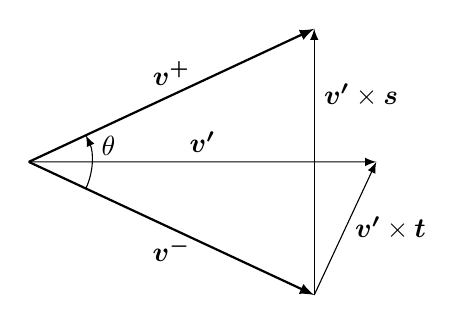
\begin{tikzpicture}[
	scale=2,
	>=latex]

	\def\centerarc[#1](#2)(#3:#4:#5)% Syntax: [draw options] (center) (initial angle:final angle:radius)
		{\draw[#1] ($(#2)+({#5*cos(#3)},{#5*sin(#3)})$) arc (#3:#4:#5); }

	\def\startangle{-25}
	\def\midangle{0}
	\def\endangle{25}
	\def\radius{2.0}
	\pgfmathsetmacro{\vlen}{\radius*tan(\startangle)}%

	\coordinate (O) at (0,0);
	\coordinate (S) at (\startangle:\radius);
	\coordinate (E) at (\endangle:\radius);

%	\centerarc[dashed](O)(\startangle:\endangle:\radius);
	\centerarc[->](O)(\startangle:\endangle:0.2*\radius);

	\draw (O)+(0.4,0.1) node [right] {$\theta$};

	\draw [thick,->] (O) -- (E) node [midway, above] {$\V{v^+}$};
	\draw [thick,->] (O) -- (S) node [midway, below] {$\V{v^-}$};

	\path (S) +(\startangle-90:\vlen) coordinate (V1E);
%	\path (E) +(\endangle-90:\vlen) coordinate (V3E);

%	%\draw [->] (E) -- (V3E);
	\draw [->] (S) -- (V1E) node [midway, right] {$\V{v'} \times \V t$};
%
	\draw [->] (O) -- (V1E) node [midway, above] {$\V{v'}$};
	\draw [->] (S) -- (E) node [near end, right] {$\V{v'} \times \V s$};

%	\draw [fill=white] (O) circle (0.02);

\end{tikzpicture}
\caption{Velocity space rotation from $\v-$ to $\v+$}
\end{figure}
%
\paragraph{Add half electric impulse} We define $\V{v^-}$ as the velocity after 
half a electric impulse:
$$\v^- = \v_{t-\dt/2} + \frac{q \E}{m} \frac{\dt}{2}$$

\paragraph{Rotate for the magnetic field} The rotation is done in two steps, 
first the half rotation is computed, with an angle of $\theta/2$:
$$\v' = \v^- + \v^- \times \V t $$

Then the rotation is completed by symmetry, using the $\V s$ vector
$$ \V s = \frac{2 \V t}{1 + \V t^2} $$
as
$$ \V{v^+} = \V{v^-} + \V{v}' \times \V{s} $$

\chapter{Parallelization}

\section{Data structures}

\chapter{Results}

\chapter{Conclusions}

%\bibliographystyle{siam}
%\bibliography{bib}

\end{document}
